\documentclass[10pt,]{article}
\usepackage{lmodern}
\usepackage{amssymb,amsmath}
\usepackage{ifxetex,ifluatex}
\usepackage{fixltx2e} % provides \textsubscript
\ifnum 0\ifxetex 1\fi\ifluatex 1\fi=0 % if pdftex
  \usepackage[T1]{fontenc}
  \usepackage[utf8]{inputenc}
\else % if luatex or xelatex
  \ifxetex
    \usepackage{mathspec}
  \else
    \usepackage{fontspec}
  \fi
  \defaultfontfeatures{Ligatures=TeX,Scale=MatchLowercase}
\fi
% use upquote if available, for straight quotes in verbatim environments
\IfFileExists{upquote.sty}{\usepackage{upquote}}{}
% use microtype if available
\IfFileExists{microtype.sty}{%
\usepackage{microtype}
\UseMicrotypeSet[protrusion]{basicmath} % disable protrusion for tt fonts
}{}
\usepackage[left=2cm, right=2cm, top=2cm, bottom=3cm, footskip = .5cm]{geometry}
\usepackage{hyperref}
\hypersetup{unicode=true,
            pdftitle={null},
            pdfborder={0 0 0},
            breaklinks=true}
\urlstyle{same}  % don't use monospace font for urls
\usepackage{graphicx,grffile}
\makeatletter
\def\maxwidth{\ifdim\Gin@nat@width>\linewidth\linewidth\else\Gin@nat@width\fi}
\def\maxheight{\ifdim\Gin@nat@height>\textheight\textheight\else\Gin@nat@height\fi}
\makeatother
% Scale images if necessary, so that they will not overflow the page
% margins by default, and it is still possible to overwrite the defaults
% using explicit options in \includegraphics[width, height, ...]{}
\setkeys{Gin}{width=\maxwidth,height=\maxheight,keepaspectratio}
\IfFileExists{parskip.sty}{%
\usepackage{parskip}
}{% else
\setlength{\parindent}{0pt}
\setlength{\parskip}{6pt plus 2pt minus 1pt}
}
\setlength{\emergencystretch}{3em}  % prevent overfull lines
\providecommand{\tightlist}{%
  \setlength{\itemsep}{0pt}\setlength{\parskip}{0pt}}
\setcounter{secnumdepth}{0}

%%% Use protect on footnotes to avoid problems with footnotes in titles
\let\rmarkdownfootnote\footnote%
\def\footnote{\protect\rmarkdownfootnote}

%%% Change title format to be more compact
\usepackage{titling}

% Create subtitle command for use in maketitle
\providecommand{\subtitle}[1]{
  \posttitle{
    \begin{center}\large#1\end{center}
    }
}

\setlength{\droptitle}{-2em}

  \title{null}
    \pretitle{\vspace{\droptitle}\centering\huge}
  \posttitle{\par}
    \author{}
    \preauthor{}\postauthor{}
    \date{}
    \predate{}\postdate{}
  
% Set up the fonts
\usepackage[urw-palatino]{mathdesign}
\usepackage[T1]{fontenc}


% Set the language for 508
\hypersetup{
  pdftitle = {title},
  pdflang = en-US}

% Add accessibility support from http://www.richschwinn.com/accessibility
\RequirePackage{accsupp}
\RequirePackage{pdfcomment}
\newcommand{\AccTool}[2]{\BeginAccSupp{method=pdfstringdef,unicode,Alt={{#1}}}\pdftooltip{{#2}}{{#1}}\EndAccSupp{}}


% Set up the headers and footers
\usepackage{graphicx}
\usepackage{fancyhdr}
\usepackage{ifthen}
\usepackage{everypage}
\usepackage{float}

% Avoid struggling over figure and table float in Rmarkdown
\let\origfigure\figure
\let\endorigfigure\endfigure
\renewenvironment{figure}[1][2] {
    \expandafter\origfigure\expandafter[H]
} {
    \endorigfigure
}

\let\origtable\table
\let\endorigtable\endtable
\renewenvironment{table}[1][2] {
    \expandafter\origtable\expandafter[H]
} {
    \endorigtable
}

% First page has the large title and NOAA logo
\pagestyle{fancy}
\fancyhf{}
\setlength\headheight{40pt}
\cfoot{\thepage}

\AddEverypageHook{%
   \ifthenelse{\value{page}=1}%
     {\rhead{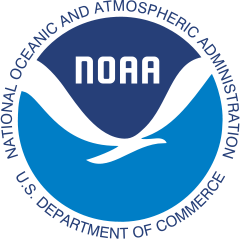
\includegraphics[width=40pt]{images/NOAA_logo.png} \\ \textsf{\emph{Published March 29, 2019}}}
      \lhead{\textsf{\LARGE State of the Ecosystem 2019: New England}}
      }%
     {\rhead{}
      \lhead{\textsf{\emph{State of the Ecosystem 2019: New England}}}
     }
}

\renewcommand{\headrulewidth}{0.4pt}
\renewcommand{\footrulewidth}{0pt}


% Change section labels to san serif
\usepackage{sectsty}
\allsectionsfont{\normalfont\sffamily\bfseries}
\usepackage{booktabs}
\usepackage{longtable}
\usepackage{array}
\usepackage{multirow}
\usepackage{wrapfig}
\usepackage{float}
\usepackage{colortbl}
\usepackage{pdflscape}
\usepackage{tabu}
\usepackage{threeparttable}
\usepackage{threeparttablex}
\usepackage[normalem]{ulem}
\usepackage{makecell}
\usepackage{xcolor}

\begin{document}
\maketitle

\section{Overview}\label{overview}

The purpose of this report is to synthesize available information
relevant to fishery management in the New England portion of the US
Northeast Shelf (the Gulf of Maine, GOM, and Georges Bank, GB). This
2019 report highlights where management interventions have proven
successful to achieve ecological objectives, but also characterizes the
considerable challenges for management posed by climate change and
increasing trade-offs across conservation, fishing, and other human
activities in this region (Fig. \ref{fig:conceptual-model}). Finally, we
describe combinations of ecological signals that present opportunities
for further integrated research and possibly creative management
solutions.

\begin{figure}

{\centering 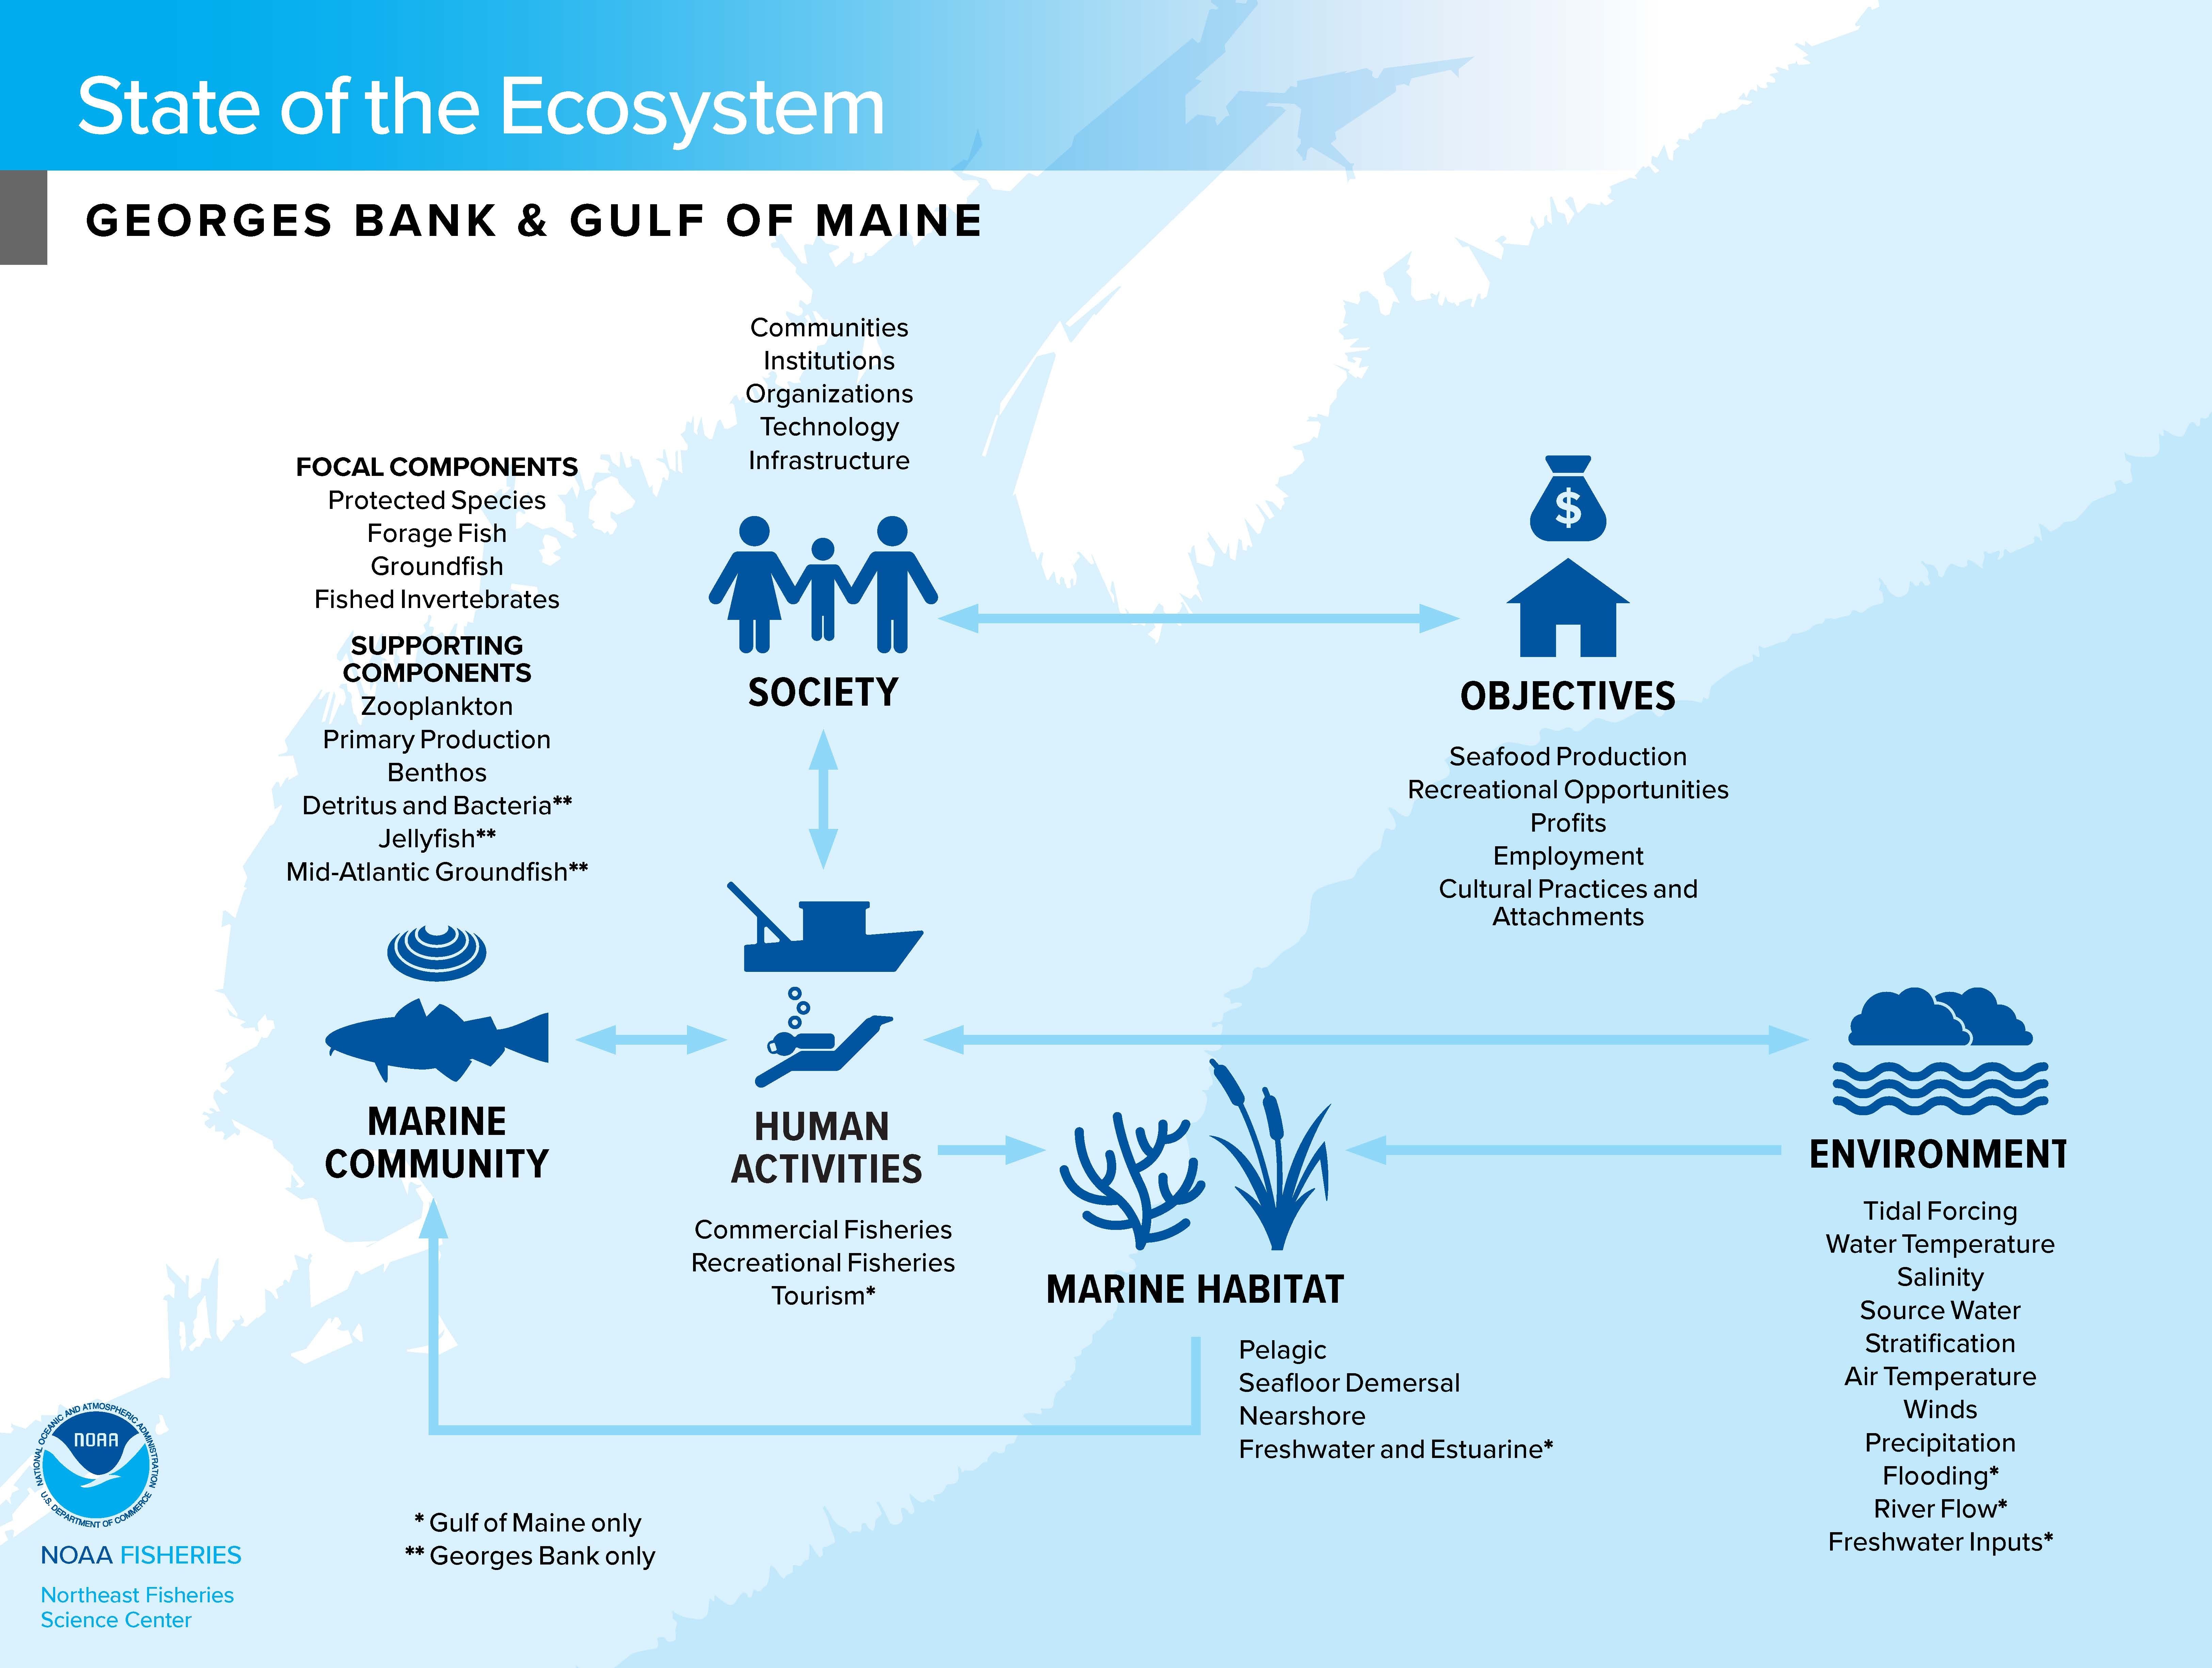
\includegraphics[width=\textwidth]{images/GOM_GB_conmod_overview} 

}

\caption{A conceptual model places detailed species-level management in context by highlighting relationships between focal species groups organized by the New England Fishery Management Council (NEFMC) Fishery Management Plan (FMP), managed human activities, environmental drivers, habitats, and key ecological links.}\label{fig:conceptual-model}
\end{figure}

Some management interventions for ecosystems and fisheries have proven
beneficial in New England and throughout the Northeast US Shelf. For
example, harbor porpoise bycatch continues to decrease. The 2016 and
2017 harbor porpoise bycatch estimates are among the lowest on record in
the Northeast US (Fig. \ref{fig:harbor-porpoise-bars}), coinciding with
an apparently stablized harbor porpoise population.

However, there are multiple signals indicating challenges to meeting
management goals. Fishery management objectives are being met for 20
stocks at the single species level, but 9 stocks are below biomass
thresholds (Fig. \ref{fig:NE-stock-status}). Both New England
social-ecological systems are reliant on a single species for the
majority of revenue (lobster in GOM, scallop in GB). These species have
moderate to high climate vulnerability, likely representing heightened
risk to fishing communities, particularly along the coast of Maine and
the South Coast of Massachusetts where ports are highly engaged and
reliant on commercial fishing (Fig.
\ref{fig:NE-comm-reliance-maps-outlined}). There are long term declines
in total seafood production and commercial revenue for New
England-managed species in the GOM (Figs. \ref{fig:comm-landings-ne},
\ref{fig:total-landings-ne}, \ref{fig:comm-revenue-ne}). However,
indicators highlight an increasing diversity of recreational species
caught in New England (Fig. \ref{fig:rec-div}).

Fisheries are significantly affecting protected species, particularly
large whale abundance. Changes in fishery management to address this
issue could have considerable consequences for the fixed gear fishing
sector, particularly for pot gear such as for lobster. The recovery of
north Atlantic right whales is affected by anthropogenic mortality (Fig.
\ref{fig:NARW-abundance}). Shifts in ecosystem conditions may be
contributing to increased interaction between right whales and fishing
gear and could be playing a role in other protected species trends.
Unusual Mortality Events (UMEs) have been declared for north Atlantic
right whales, humpback whales, and minke whales, and preliminary
investigations suggest fishing gear entanglement has played a primary
role in these mortalities. Gray seal bycatch mortality has also risen in
recent years, with an estimated annual mortality that has often totaled
more than 1000 animals and a UME has been declared for both gray and
harbor seals that may be due to phocine distemper virus.

Several climate and ecosystem observations are trending towards or have
reached unprecedented levels. The Northeast US shelf is among the
fastest warming waters globally (Fig. \ref{fig:long-term-sst}) with
implications for species physiology, productivity, distribution, and
community composition. Globally, 2018 was the 4th warmest year on record
with the last four years being the warmest on record. In both the GOM
and GB, 2018 seasonal sea surface temperatures were above average, while
while the summer temperatures in the Gulf of Maine were the highest on
record (Fig. \ref{fig:NE-SST-anom-series}). Annual average bottom
temperature measurements show a significant long term warming trend in
the GOM (Fig. \ref{fig:NE-bot-temp}). Ocean circulation is changing as
well. The position of the northern edge of the Gulf Stream has trended
northward since the late 1950s, with an increasing rate since 2009. The
most northerly positions on record were observed between 2014-2017 (Fig.
\ref{fig:GSI}). Since the mid-2000'??s, the warmer, saltier shelf slope
water associated with the Gulf Stream has dominated the input into the
GOM at the Northeast Channel (Fig. \ref{fig:wsw-prop}). A more northerly
Gulf Stream position is generally associated with warmer ocean
temperature in the Northeast US shelf
{[}\protect\hyperlink{ref-zhang_role_2007}{1}{]} and increased sea
surface height along the U.S. east coast
{[}\protect\hyperlink{ref-goddard_extreme_2015}{2}{]}.

The management implications of these ocean changes vary by region and
species, and are not fully understood at this point. Changes in the
distribution of managed fish species continue, with aggregate trends on
the entire Northeast Shelf shifting towards the northeast and generally
into deeper water (Fig. \ref{fig:spec-dist}). These shifts place
increasing pressure on the management system. The proportion of NEFMC
managed benthivore species (righteye flounders, haddock) has declined
over time in Mid-Atlantic waters according to bottom trawl surveys (Fig.
\ref{fig:NEFMC-in-MAB}), while the proportion of MAFMC managed
planktivore (squids, mackerel, and butterfish) species has been
increasing in New England waters in both surveys and landings (Figs.
\ref{fig:MAFMC-in-NE}, \ref{fig:comm-landings-ne}). Butterfish have been
observed in Gulf of Maine common tern fledgling diets between 2009-2011
and again in 2018 (Fig. \ref{fig:map-and-prey}b), which negatively
impacts tern productivity. The downward trend in recreational species
diversity in the Mid-Atlantic (see Mid-Atlantic report) contrasts with
an increase in recreational species diversity over time in New England
(Fig. \ref{fig:rec-div}), although it is unclear to what extent this
result is due to the aggregation of SAFMC species in the indicator
itself. Nearshore MA and ME/NH survey indices show some similar patterns
to offshore surveys, although with different magnitudes, perhaps
reflecting seasonal importance of nearshore habitats (Figs.
\ref{fig:gom-biomass-ne}, \ref{fig:MA-inshore}, \ref{fig:menh-survey});
these patterns will be explored in more detail in future analyses. As
temperature and ocean circulation indicators trend toward extremes,
fishery management based on static stock areas will likely face
continued changes in species distribution.

Observed changes at the base of the food web, including timing and
community composition, affect productivity of protected and managed
species in ways we do not yet fully understand. There is a trend of
increasing primary production in New England, but this trend is
primarily driven by increased summer production, which is due to warmer
temperatures and increased bacterial remineralization and nutrient
recycling (Fig. \ref{fig:NE-PP-OCCI}). This increased productivity is
most likely from smaller-celled species that contribute less to fish
production compared to larger phytoplankton. Current zooplankton trends
show a shift towards smaller-bodied copepods (Fig. \ref{fig:NE-sli}).
This suggests a possible return to conditions last observed during the
1990s, when small bodied copepods dominated the zooplankton community,
regime shifts in groundfish recruitment were observed
{[}\protect\hyperlink{ref-perretti_regime_2017}{3}{]}, and north
Atlantic right whales experienced lower birth rates
{[}\protect\hyperlink{ref-greene_remote_2013}{4}{]}. The timing of
shifts in fish condition may be similar (Fig. \ref{fig:ne-cf}), though
potential mechanisms connecting adult fish condition to zooplankton
patterns require further study.

\section{Report Structure}\label{report-structure}

The major messages of the report are synthesized above with reference to
key figures. The information in this report is organized around general
ecosystem-level management objectives (Table
\ref{tab:management-objectives}), and indicators related to these
objectives are grouped into four general categories in the four sections
below: economic and social, protected species, fish and invertebrates,
and habitat quality and ecosystem productivity. Each section begins with
a summary of main messages with links to other sections, including any
new information added at the request of the Council, and includes
figures with brief descriptions of all current indicators. Detailed
technical methods documentation\footnote{\url{https://NOAA-EDAB.github.io/tech-doc}}
and indicator data\footnote{\url{https://github.com/NOAA-EDAB/ecodata}}
are available online. The details of standard figure formatting (Fig.
\ref{fig:docformat}a), categorization of fish and invertebrate species
into feeding groups (Table \ref{tab:species-groupings}), and definitions
of ecological production units (EPUs, including the Gulf of Maine (GOM)
and Georges Bank (GB); Fig. \ref{fig:docformat}b) are provided at the
end of the document.

\begin{table}[!h]

\caption{\label{tab:management-objectives}Established ecosystem-scale objectives in New England}
\centering
\begin{tabular}{ll}
\toprule
\textbf{Objective Categories} & \textbf{Indicators reported here}\\
\midrule
Seafood Production & Landings by feeding guild\\
Profits & Revenue by feeding guild\\
Recreation & Number of anglers and trips; recreational catch\\
Stability & Diversity indices (fishery and species)\\
Social \& Cultural & Commercial and recreational reliance\\
\addlinespace
Biomass & Biomass or abundance by feeding guild from surveys\\
Productivity & Condition and recruitment of MAFMC managed species\\
Trophic structure & Relative biomass of feeding guilds, primary productivity\\
Habitat & Estuarine and offshore habitat conditions\\
\bottomrule
\end{tabular}
\end{table}

\section{Economic and Social}\label{economic-and-social}

The objectives of U.S. federal fishery management include providing
benefits to the Nation in terms of seafood production and recreational
opportunities, while considering economic efficiency and effects on
coastal communities. The indicators in this section consider these
objectives for the GOM and GB ecological production units separately
where possible.

\subsection{Gulf of Maine}\label{gulf-of-maine}

A long term significant decrease in NEFMC managed species revenue was
offset by non-NEFMC managed species (Fig. \ref{fig:comm-revenue-ne}),
likely lobster, as indicated by the focal component-level Bennet Volume
Indicator for Benthivores (Fig. \ref{fig:bennet-ne}).

\begin{figure}

{\centering \includegraphics{SOE-NEFMC-2019_files/figure-latex/comm-revenue-ne-1} 

}

\caption{Total commercial revenue (black) and revenue from NEFMC managed species (red) in Gulf of Maine (left) and Georges Bank (right).}\label{fig:comm-revenue-ne}
\end{figure}

\begin{figure}

{\centering \includegraphics{SOE-NEFMC-2019_files/figure-latex/bennet-ne-1} 

}

\caption{Revenue change from the long-term mean in 2015 dollars (black), Price (PI), and Volume Indicators (VI) for commercial benthivore landings in Gulf of Maine (left) and for commercial benthos landings on Georges Bank (right).}\label{fig:bennet-ne}
\end{figure}

There is a concurrent significant decrease in NEFMC-managed commercial
seafood production and landings (Fig. \ref{fig:total-landings-ne}), with
Piscivores, Planktivores, and NEFMC-managed Benthivores showing long
term negative trends (Fig. \ref{fig:comm-landings-ne}). This trend is a
continuation on the reliance on a small number of species, which could
induce additional risk in the social system.

\begin{figure}

{\centering \includegraphics{SOE-NEFMC-2019_files/figure-latex/total-landings-ne-1} 

}

\caption{Total commercial seafood landings (black) shown with NEFMC managed seafood landings (red) in Gulf of Maine (left) and Georges Bank (right).}\label{fig:total-landings-ne}
\end{figure}

One notable signal suggesting increased importance of non-NEFMC managed
species is the divergence between NEFMC managed and non-NEFMC managed
Planktivore landings in last 5 years in the GOM (Fig.
\ref{fig:comm-landings-ne}), the result of lower Atlantic herring
landings relative to other planktivores. Additionally, the importance of
state-managed fisheries continues to increase, with highly dependant and
thus highly vulnerable ports in Maine relying on lobster.

\begin{figure}

{\centering \includegraphics{SOE-NEFMC-2019_files/figure-latex/comm-landings-ne-1} 

}

\caption{NEFMC managed species landings (red) and total commercial landings (black) by feeding guild in Gulf of Maine (left) and Georges Bank (right).}\label{fig:comm-landings-ne}
\end{figure}

\subsection{Georges Bank}\label{georges-bank}

In contrast with the GOM, GB total landings and revenue have no long
term trends for NEFMC-managed species (Fig.
\ref{fig:total-landings-ne}). Rather, fluctuations in GB total revenue
and in particular benthos landings (Fig. \ref{fig:comm-landings-ne}) may
be associated with rotational management for scallops altering effort
between the GB and MAB ecological production units. Planktivore landings
on GB have increased over the long term, but have returned to the long
term average in 2017. Price and volume components of revenue are both
lower since 2015 (slightly down from the long-run average, Fig.
\ref{fig:bennet-ne}), driven by generally decreased landings and despite
improved Benthivore, Other, and Planktivore prices. Scallop revenue
continues to play an oversized role in Georges Bank dynamics.

\subsection{New England-wide}\label{new-england-wide}

New England social-ecological systems are each reliant on a single
crustacean or shellfish species for the majority of commercial fisheries
revenue (lobster in GOM, scallop in GB). This reliance likely represents
heightened risk to fishing communities, particularly along the coast of
Maine and the South Coast in MA in ports which are highly engaged and
reliant on commercial fishing (Fig.
\ref{fig:NE-comm-reliance-maps-outlined}). This risk is heightened by
the moderate to high climate vulnerability of crustaceans and shellfish,
which face risks from ocean acidification as well as increased
temperature {[}\protect\hyperlink{ref-hare_vulnerability_2016}{5}{]}.

\begin{figure}

{\centering \includegraphics{SOE-NEFMC-2019_files/figure-latex/NE-comm-reliance-maps-outlined-1} 

}

\caption{Commercial engagement (total pounds landed, value landed, commercial permits and commercial dealers in a community) and reliance (per capita engagement) based on 2016 landings and the ACS running average of 2012-2016 census data.}\label{fig:NE-comm-reliance-maps-outlined}
\end{figure}

Commercial fleet diversity indices were updated with 2017 data. Current
diversity remains near the long term average.

In contrast to commercial species specialization, indicators highlight
an increasing diversity of recreational species caught in New England
(Fig. \ref{fig:rec-div}), although recreational fleet effort diversity
has not changed over the long term.

\begin{figure}

{\centering \includegraphics{SOE-NEFMC-2019_files/figure-latex/rec-div-1} 

}

\caption{Recreational effort diversity and diversity of recreational catch in the New England.}\label{fig:rec-div}
\end{figure}

Recreational seafood production shows an increasing trend since the
mid-1990s with the updated Marine Recreational Information Program
(MRIP) data (Fig. \ref{fig:rec-landings-ne})).

\begin{figure}

{\centering \includegraphics{SOE-NEFMC-2019_files/figure-latex/rec-landings-ne-1} 

}

\caption{Total recreational seafood harvest in New England.}\label{fig:rec-landings-ne}
\end{figure}

Updated indicators for recreational opportunities (effort days and
number of anglers) show general increases since the 1990s, peaking in
the late 2000s and declining since then. This is similar to previously
reported trends (Fig. \ref{fig:rec-op}). All recreational indicators
have been updated with new MRIP data, and indicators for recreational
diversity are new for this report.

\begin{figure}

{\centering \includegraphics{SOE-NEFMC-2019_files/figure-latex/rec-op-1} 

}

\caption{Recreational effort and number of recreational anglers in the New England.}\label{fig:rec-op}
\end{figure}

Recreational fishing is important to many New England communities,
particularly in Southern New England (MA, RI, CT; Fig.
\ref{fig:NE-rec-engage}). Communities that are most socially and
economically dependent (both engaged and reliant) on recreational
fishing may benefit from the increased diversity of recreational species
catch. Additional social indicators for New England communities are
available online\footnote{\url{https://www.st.nmfs.noaa.gov/humandimensions/social-indicators/}}.

\begin{figure}

{\centering \includegraphics{SOE-NEFMC-2019_files/figure-latex/NE-rec-engage-1} 

}

\caption{Recreational engagement (shore, private vessel and for-hire recreational fishing in a community) and reliance (per capita engagement) based on 2016 landings and the ACS running average of 2012-2016 census data.}\label{fig:NE-rec-engage}
\end{figure}

\newpage

\section{Protected Species}\label{protected-species}

Protected species include marine mammals (under the Marine Mammal
Protection Act), endangered and threatened species (under the Endangered
Species Act), and migratory birds (under the Migratory Bird Treaty Act).
In the Northeast US, endangered/threatened species include Atlantic
salmon, Atlantic and shortnose sturgeon, all sea turtle species, and 5
baleen whales. Fishery management objectives for protected species
generally focus on reducing threats and on habitat
conservation/restoration; here we report on the status of these actions
as well as indicating the potential for future interactions driven by
observed and predicted ecosystem changes in the Northeast US region.
Atlantic salmon are among the most critically endangered fish and are a
NOAA Species in the Spotlight. This year four Unusual Mortality Events
(UMEs) have been declared for three large whale species and two seal
species, with several mortalities attributed to human interactions.
Also, a marine mammal climate vulnerability assessment is currently
underway for Atlantic and Gulf of Mexico populations and will be
reported on in future versions of this report. Strong evidence exists to
suggest that the level of interaction between right whales and the
combination of fixed gear in the US and Canada is contributing
substantially to the decline of the species.

\subsection{Sea turtles (coastwide)}\label{sea-turtles-coastwide}

Sea turtles are known to be susceptible to climate and ecosystem
changes, and their distribution is influenced by water temperature. Sea
turtle diets contain a considerable amount of gelatinous zooplankton,
which are also influenced by changes in the ecosystem. At present,
management measures to reduce sea turtle-fishery interactions are
limited to the regions with historical observations of sea turtles and
based on historical ocean temperature distributions. However, changes in
climate may cause turtles to shift northward into areas with heavy
fishing, possibly resulting in increased bycatch. It has been
hypothesized that seasonal distribution of Kempas Ridley sea turtles has
shifted northward due to the warming of the Gulf of Maine, which in
turn, appears to be resulting in a near record number of cold-stunned
turtles stranding in Cape Cod Bay as waters cooled during the fall of
2018.

\subsection{Whales (coastwide)}\label{whales-coastwide}

North Atlantic right whales are among the most endangered large whale
populations in the world. Changes in right whale trends can have
implications for fisheries management where fisheries interact with
these whales. Additional management restrictions could have a large
impact on fishing times, gears, etc. Although the population increased
steadily from 1990 to 2011, it has decreased recently (Fig.
\ref{fig:NARW-abundance}). From
{[}\protect\hyperlink{ref-pace_statespace_2017}{6}{]}: `??The
probability that the population'??s trajectory post-2010 was a decline
was estimated at 99.99\%.'?? Reduced survival rates of adult females and
diverging abundance trends between sexes have also been observed. It is
estimated that there are only about 100 adult females remaining in the
population. Further, right whale distribution has changed since 2010.
The reasons for these changes is unclear, but changes in climate and
primary prey (\emph{Calanus finmarchicus}) are suspected.

Three large whale Unusual Mortality Events (UMEs) have been declared for
north Atlantic right whales, humpback whales, and minke whales. In all
three cases human interaction appears to have contributed to increased
mortalities, although investigations are not complete. Twenty right
whale mortalities have been documented in 2017 and 2018 so far. Among
the 20 right whale deaths observed in 2017 and 2018 thus far, 5 were due
to vessel strike (1 in US waters, 4 in Canadian waters), 6 from
entanglement (2 in Canadian gear, 1 in unknown gear, and 3 others found
in US waters), and the rest from unknown causes. UMEs have also been
declared for humpback whales during 2016-2018 and 2017-2018 minke whales
due to elevated strandings. Necropsy investigations on 50\% of humpback
whales showed evidence of human interaction, either ship strike or
entanglement. Similarly, 60\% of minke whales show evidence of human
interactions or infectious disease. In both cases the investigations are
still underway and more research is needed to determine the causes of
these UME.

\begin{figure}

{\centering \includegraphics{SOE-NEFMC-2019_files/figure-latex/NARW-abundance-1} 

}

\caption{Right whale abundance estimates with 95\% credible intervals. These values represent the estimated number of animals alive sometime during the year referenced and NOT at the end of the year referenced. Seventeen known deaths were recorded in 2017 (likely all from anthropogenic causes), but these deaths were not reflected in the 2017 estimate because those animals were alive sometime during the year.}\label{fig:NARW-abundance}
\end{figure}

\subsection{Grey seals (coastwide)}\label{grey-seals-coastwide}

The number of grey seals (\emph{Halichoerus grypus}) in U.S. waters has
risen dramatically in the last 2 decades, with few observed in the early
1990s to roughly 24,000 observed in southeastern Massachusetts in 2015
(Pace et al. in press). Roughly 30,000 - 40,000 gray seals were
estimated in southeastern Massachusetts in 2015, using correction
factors applied to seal counts visible in Google Earth imagery. As of
2016, the size of the grey seal population in Canada, which is part of
the same stock as the grey seals in the U.S., was estimated to be
roughly 425,000, and increasing by 4\% a year. Pups born on Muskeget
Island MA, currently the largest pupping site for gray seals in the
U.S., were first observed in 1988 and now number over 3,500. Trends in
pup production at U.S. colonies appear to be increasing, and it is
likely that U.S. pup production is being supplemented each year by
animals from Canada. A UME for both gray and harbor seals was declared
in 2018, triggering an investigation into the cause of this event. Tests
so far suggest phocine distemper virus as a potential cause, although
the investigation is not yet complete.

Fisheries interactions have increased over the past 2 decades, with
fewer than 10 total estimated grey seal interactions in 1993, to more
than 1000 in 2013 and 2015, and with the preliminary 2017 estimate over
900. Analysis of seal diet is currently underway using a variety of
techniques (analysis of stomach contents, fatty acids, and DNA) to
assess the potential impact of seal population growth on the ecosystem
and important commercial fish species.

\subsection{Harbor porpoise
(coastwide)}\label{harbor-porpoise-coastwide}

Harbor porpoise bycatch has resulted in fisheries closures in the past,
but current bycatch levels suggest that management measures have been
effective, reducing this fishery interaction. The 5-year mean bycatch
has been below the maximum permitted level (Potential Biological
Removal, PBR) since 2011 (Fig. \ref{fig:harbor-porpoise-bars}), and the
2016 and draft 2017 annual bycatch estimates are among the lowest in the
time series. Recent compliance with the harbor porpoise take reduction
plan and reduced fishing effort are thought to contribute to low bycatch
estimates. Potential recent shifts in porpoise distribution could also
be contributing to low bycatch and this will be explored during the
coming year. A new draft harbor porpoise abundance estimate suggests
stable or increasing abundance of the Gulf of Maine/Bay of Fundy harbor
porpoise stock. Recent analyses have examined regional harbor porpoise
diet, and suggest that harbor porpoise are not typically feeding on fish
caught in gillnets. However, the impact of ecosystem changes on bycatch,
population, or distribution remain unclear.

\begin{figure}

{\centering \includegraphics{SOE-NEFMC-2019_files/figure-latex/harbor-porpoise-bars-1} 

}

\caption{Harbor porpoise bycatch estimate (black) shown with Potential Biological Removal (red). Error bars indicate 95\% confidence interval.}\label{fig:harbor-porpoise-bars}
\end{figure}

\subsection{Protected fish (coastwide)}\label{protected-fish-coastwide}

The Gulf of Maine DPS of Atlantic salmon is listed as endangered. These
salmon are found in coastal waters of New England and now spawn only in
Maine rivers. Spawner abundance is less than 10\% of historic levels
with returns averaging around 1,000 annually since 2012. They are highly
reliant on connectivity between ocean and freshwater habitats to
complete their life cycle. They are also extremely sensitive to climate
and ecosystem changes since they have specific habitat requirements for
each of their life stages. These populations migrate through some of the
most rapidly warming marine regions and marine regime shifts have
impacted their ocean productivity. The Recovery Plan for the Gulf of
Maine DPS of Atlantic Salmon was published in 2019, and it highlights
specific actions to conserve and recover the species: enhancing
river-ocean connectivity; maintaining genetic diversity; increasing the
number of spawning adults; and furthering our understanding of marine
and estuarine habitats. Shortnose sturgeon (endangered) and five
distinct populations segments (DPS) of Atlantic sturgeon are found in
coastal waters of New England (endangered: New York Bight, Chesapeake
Bay, Carolina, and South Atlantic; threatened: Gulf of Maine). Several
populations spawn in New England watersheds, and river-ocean
connectivity is an important habitat characteristic. These populations
are vulnerable to climate and ecosystem changes as their life history
results in high biological sensitivity and habitat needs result in very
high climate exposure. Threat reductions are focused on protecting
critical habitat, habitat restoration, reducing ship-strikes, and
bycatch reduction.

\subsection{Common terns (GOM)}\label{common-terns-gom}

Seabird breeding colonies in the GOM are monitored and managed to
promote recovery of formerly harvested species. Common terns are
well-monitored and are considered good nearshore ecosystem indictators
due to their wide distribution and generalist diet. Common terns breed
on islands throughout the Gulf of Maine (Fig. \ref{fig:map-and-prey}a),
feeding on a wide range of invertebrates and fish including Atlantic
herring, juvenile (mainly white) hakes, and sand lance (Fig.
\ref{fig:map-and-prey}b). As surface feeding birds, terns are sensitive
to vertical distribution of prey as well as nearshore conditions in
general, with a foraging distance of 10-20 km from a nesting colony.

\begin{figure}

{\centering \includegraphics{SOE-NEFMC-2019_files/figure-latex/map-and-prey-1} 

}

\caption{Common terns: a. Locations of the seven sampled common tern nesting sites in Gulf of Maine (EER = Eastern Egg Rock, JI = Jenny Island, MR = Matinicus Rock, OGI = Outer Green Island, PINWR = Pond Island National Wildlife Refuge, SINWR = Seal Island National Wildlife Refuge, STI = Stratton Island), and b. Prey frequencies in the diets of common tern observed across the seven colonies in Gulf of Maine. Prey occurring in <5 percent of common tern diets were excluded for clarity.}\label{fig:map-and-prey}
\end{figure}

GOM common tern average productivity (fledglings per nest) across 7
colonies has varied over time but was low in 2018 (Fig.
\ref{fig:tern-prod-div}a), a year with record-high summer SST in the GOM
(Fig. \ref{fig:NE-SST-anom-series}), and substantial butterfish in tern
diets (Fig. \ref{fig:map-and-prey}b).

\begin{figure}

{\centering \includegraphics{SOE-NEFMC-2019_files/figure-latex/tern-prod-div-1} 

}

\caption{a. Mean common tern productivity at nesting sites in Gulf of Maine. Error bars show +/- 1 SE of the mean. b. Shannon diversity of common tern diets observed at nesting sites in Gulf of Maine. Diversity of common tern diets has been predominantly above the long-term mean since 2006.}\label{fig:tern-prod-div}
\end{figure}

The presence of butterfish in tern diets reflects the extension of this
warm water species into GOM. Due to their thin, deep body form,
butterfish are often difficult for small seabird chicks to ingest and
swallow, causing chicks to starve and/or parent birds to increase
foraging effort. GOM common tern diet diversity was mainly above the
long term mean since 2006 (Fig. \ref{fig:tern-prod-div}b). High diet
diversity may be related to lower availability of preferred prey types
such as herring and sand lance relative to increased availability of
other species associated with warmer SST.

\newpage

\section{Fish and Invertebrates}\label{fish-and-invertebrates}

Fishery management aims to keep individual harvested species within
population ranges where productivity is maximized over the long-term.
However, these managed species represent a subset of the full ecosystem,
interacting with a wider range of predators and prey and relying on
diverse habitats. Indicators in this section summarize single species
status as well as tracking trends for broad categories of fish within
the ecosystem, including changes in biomass, distribution, condition,
and diversity. Changes in overall predator and prey levels as well as
distribution have implications for managed fish productivity, fishing
operations, and regional fishery management.

\subsection{Stock status and aggregate distribution
(coastwide)}\label{stock-status-and-aggregate-distribution-coastwide}

Fishery management objectives are being met for 20 (including 6 skate)
stocks at the single species level. Stocks in Fig.
\ref{fig:NE-stock-status} which are above the F threshold (horizontal
line) are experiencing overfishing (F \textgreater{} Fmsy). Stocks in
Fig. \ref{fig:NE-stock-status} which are below the B threshold (dashed
vertical line) are overfished (B \textless{} 0.5Bmsy). For the stocks
with either missing F or B values in Fig. \ref{fig:NE-stock-status},
additional information has been used to determine overfishing and
overfished status. Official stock status for New England
stocks\footnote{\url{https://www.st.nmfs.noaa.gov/sisPortal/mapTool.jsp}}
lists 6 stocks subject to overfishing (GOM cod, GB cod, southern red
hake, and all 3 yellowtail flounder stocks), and 13 stocks as overfished
(GOM cod, GB cod, southern red hake, Atlantic halibut, Atlantic
wolffish, ocean pout, thorny skate, GOM/GB windowpane flounder, southern
New England/mid-Atlantic winter flounder, witch flounder, and all 3
yellowtail flounder stocks). Five stocks have unknown status for B and
F.

\begin{figure}

{\centering \includegraphics{SOE-NEFMC-2019_files/figure-latex/NE-stock-status-1} 

}

\caption{Summary of single species status for NEFMC and jointly managed stocks. \label{stock-status}}\label{fig:NE-stock-status}
\end{figure}

Changes in the distribution of managed fish species continue, with
aggregate trends on the entire Northeast Shelf towards the northeast and
generally into deeper water (Fig. \ref{fig:spec-dist}). These shifts
will place increasing pressure on a management system based around
stable species distributions.

\begin{figure}

{\centering \includegraphics{SOE-NEFMC-2019_files/figure-latex/spec-dist-1} 

}

\caption{Aggregate species distribution metrics for species in the Northeast Large Marine Ecosystem.}\label{fig:spec-dist}
\end{figure}

\subsection{Survey biomass (GOM and
GB)}\label{survey-biomass-gom-and-gb}

Biomass across trophic levels shows similar trends between the Gulf of
Maine and Georges Bank offshore, but nearshore trends differ for some
groups. For both the GOM and GB, there are long term increasing trends
in aggregate NEFSC (offshore) survey biomass for Piscivores,
Planktivores and Benthos in the fall. (Figs. \ref{fig:gom-biomass-ne},
\ref{fig:gb-biomass-ne}). GB spring Benthos and GOM spring Planktivores
are also increasing over the long term. However, there are some notable
departures from these trends recently.

\begin{figure}

{\centering \includegraphics{SOE-NEFMC-2019_files/figure-latex/gom-biomass-ne-1} 

}

\caption{Fall (left) and spring (right) NEFSC surveyed biomass in the Gulf of Maine.}\label{fig:gom-biomass-ne}
\end{figure}

\begin{figure}

{\centering \includegraphics{SOE-NEFMC-2019_files/figure-latex/gb-biomass-ne-1} 

}

\caption{Fall (left) and spring (right) NEFSC surveyed biomass on Georges Bank.}\label{fig:gb-biomass-ne}
\end{figure}

Benthivore biomass catch in both offshore surveys has shown recent
declines from 2015 highs in both fall and spring. This contrasts with
inshore surveys showing more stable Benthivore biomass in the past few
years (Figs \ref{fig:MA-inshore}, \ref{fig:menh-survey}). Change in
haddock catch is the largest contributor to these fluctuations.

\begin{figure}

{\centering \includegraphics{SOE-NEFMC-2019_files/figure-latex/MA-inshore-1} 

}

\caption{Fall (left) and spring (right) surveyed biomass from the MA state inshore bottom trawl survey.}\label{fig:MA-inshore}
\end{figure}

\begin{figure}

{\centering \includegraphics{SOE-NEFMC-2019_files/figure-latex/menh-survey-1} 

}

\caption{Fall (left) and spring (right) surveyed biomass from the ME/NH state inshore bottom trawl survey.}\label{fig:menh-survey}
\end{figure}

Fall offshore benthivore levels remain high in the Gulf of Maine (Fig.
\ref{fig:gom-biomass-ne}), however, the New Hampshire/Maine survey shows
a recent decline (Fig. \ref{fig:menh-survey}). Fall offshore planktivore
levels returned towards the time series mean in the Gulf of Maine after
two high years.

All fall aggregate groups on Georges Bank are at or below their time
series mean for the offshore survey (Fig. \ref{fig:gb-biomass-ne}).
Spring benthos biomass levels remain high on Georges Bank, and show
significant increases over the long-term.

The proportion of NEFMC managed benthivore species (righteye flounders,
haddock) has declined over time in Mid-Atlantic waters according to
bottom trawl surveys (Fig. \ref{fig:NEFMC-in-MAB}), while the proportion
of MAFMC managed planktivore (squids, mackerel and butterfish) species
has been increasing in New England waters in both surveys and landings
(Fig. \ref{fig:MAFMC-in-NE}, Fig. \ref{fig:comm-landings-ne}).

\begin{figure}

{\centering \includegraphics{SOE-NEFMC-2019_files/figure-latex/NEFMC-in-MAB-1} 

}

\caption{New England-managed survey proportion of MAB benthivores.}\label{fig:NEFMC-in-MAB}
\end{figure}

\begin{figure}

{\centering \includegraphics{SOE-NEFMC-2019_files/figure-latex/MAFMC-in-NE-1} 

}

\caption{Mid-Atlantic-managed survey proportion of GOM and GB planktivores.}\label{fig:MAFMC-in-NE}
\end{figure}

Other observations corroborate these survey trends. For example,
butterfish have been observed in Gulf of Maine common tern fledgling
diets between 2009-2011 and again in 2018 (Fig.
\ref{fig:map-and-prey}b). The downward trend in recreational species
diversity in the Mid-Atlantic (see Mid-Atlantic report) contrasts with
an increase in recreational species diversity over time in New England
(Fig. \ref{fig:rec-div}), although it is unclear to what extent this
result is due to the aggregation of SAFMC species in the indicator
itself. As temperature and ocean circulation indicators trend toward
extremes (next section), fishery management will likely face continued
changes in species distribution.

\subsection{Fish condition (coastwide, NEFMC managed
stocks)}\label{fish-condition-coastwide-nefmc-managed-stocks}

Fish condition is measured as the weight at a given length relative to
the average - a measure of afatnessa, and a factor that influences
fecundity. This information is from fall NEFSC bottom trawl surveys.
Overall, condition factor has improved for many New England species
since 2012, similar to overall high condition prior to 2000, and in
contrast to overall lower condition between 2001-2010 (Fig.
\ref{fig:ne-cf}). The timing of these shifts is similar to shifts in the
small-large zooplankton indicator (Fig. \ref{fig:NE-sli}). Condition
factor for some NEFMC managed species (red hake, GOM haddock, ocean
pout, spiny dogfish, thorny skates, and components of winter, yellowtail
and windowpane flounder stocks) was high in 2018.

\begin{figure}

{\centering 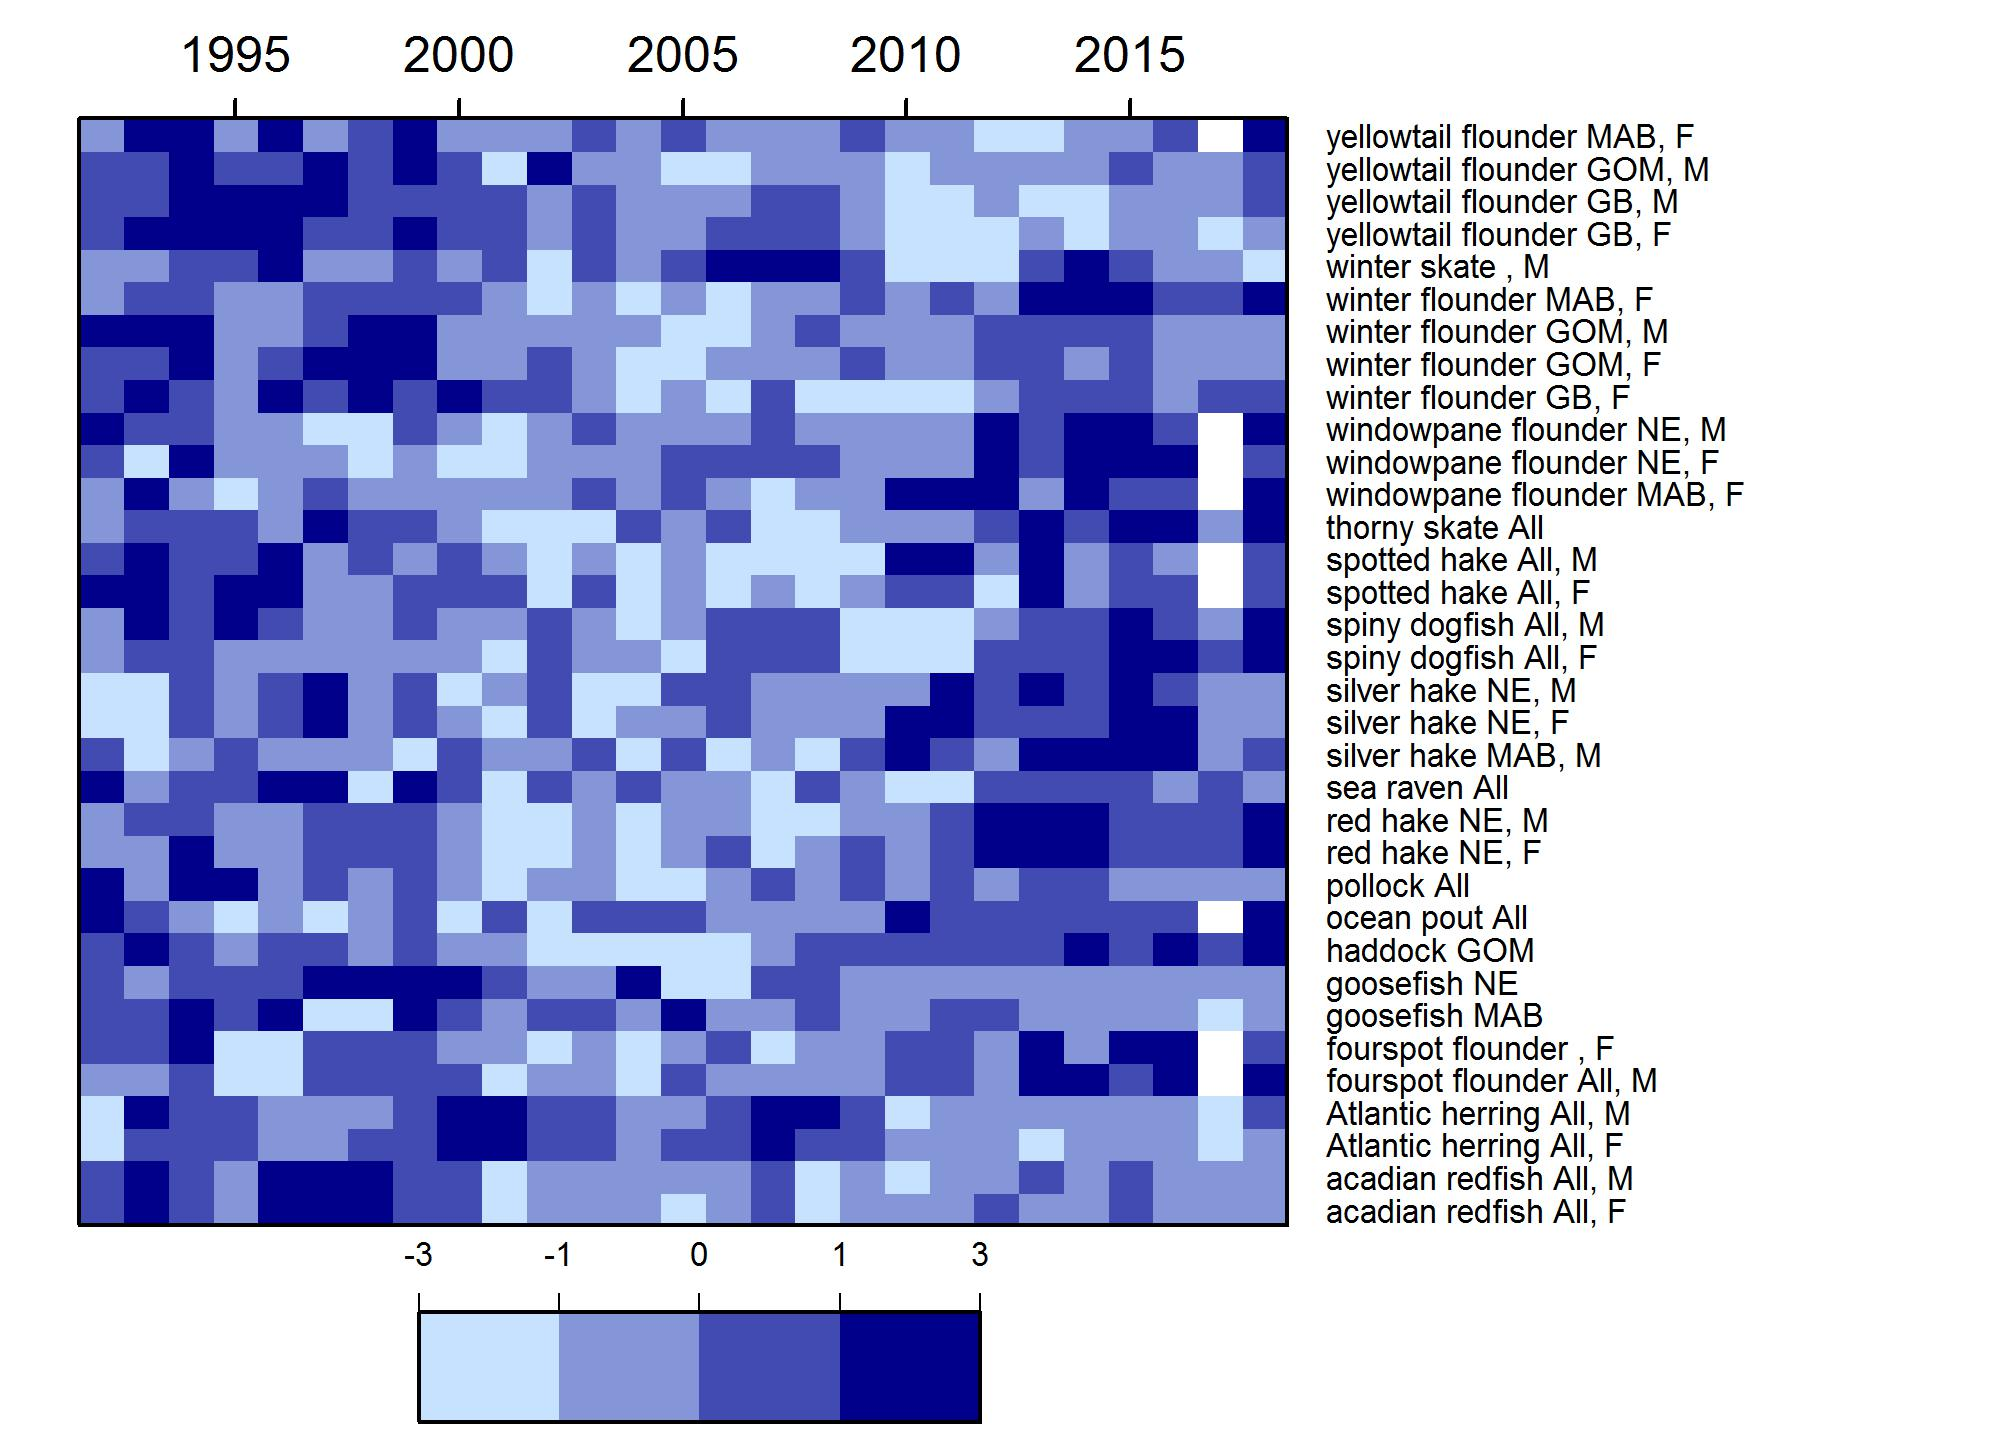
\includegraphics[width=\textwidth]{C:/Users/kimberly.bastille/Documents/GitHub/SOE-NEFMC/images/NEFMC_Fish_Condition_2019} 

}

\caption{Condition factor for NEFMC managed species.}\label{fig:ne-cf}
\end{figure}

\subsection{Larval diversity (GOM and
GB)}\label{larval-diversity-gom-and-gb}

Fluctuations in larval diversity from NEFSC ECOMON and bottom trawl
surveys reflect changing dominance of forage fish, hake, and haddock.
GOM larval diversity has been difficult to track due to poor recent
ECOMON survey coverage in the winter (Fig. \ref{fig:gom-larval-div}). GB
spring larval diversity and richness were relatively low in 2017 (the
most recent year with adequate coverage) due to high larval abundance of
haddock and sand lance (Fig. \ref{fig:gb-larval-div}).

\begin{figure}

{\centering \includegraphics{SOE-NEFMC-2019_files/figure-latex/gom-larval-div-1} 

}

\caption{Larval diversity indices from ECOMON surveys in the Gulf of Maine.}\label{fig:gom-larval-div}
\end{figure}

\begin{figure}

{\centering \includegraphics{SOE-NEFMC-2019_files/figure-latex/gb-larval-div-1} 

}

\caption{Larval diversity indices from ECOMON surveys on Georges Bank.}\label{fig:gb-larval-div}
\end{figure}

Investigations are underway to evaluate changes in timing of spawning
for managed fish species. Preliminary work with New England flatfishes
suggests that some inshore stocks are spawning earlier as temperatures
increase. There are implications for changes in spawning timing for fish
condition and for larval survival as match or mismatch with zooplankton
food sources changes (next section).

\newpage

\section{Habitat Quality and Ecosystem
Productivity}\label{habitat-quality-and-ecosystem-productivity}

Productivity of harvested fish and protected species, and therefore
sustainability of fisheries, depends on adequate habitat. Habitat
encompasses physical, chemical, and biological factors, including
biological productivity at the base of the food web. Many harvested and
protected species on the Northeast US shelf occupy several distinct
habitats throughout their life cycle, including estuaries, nearshore
coastal, and offshore environments. The indicators in this section
provide information on the changing conditions encountered by managed
species in different seasons and across habitats, which may explain
observed changes in species distribution and productivity. Ultimately, a
better understanding of these ecological drivers may permit proactive
management in a changing system.

Ocean temperatures in coastal and offshore habitats are at or near
unprecedented levels, accompanied by alterations in ocean circulation
patterns. Observed changes at the base of the food web, including timing
of production and plankton community composition, affect productivity of
protected and managed species in ways we do not yet fully understand.

\subsection{Ocean circulation and surface temperature
(coastwide)}\label{ocean-circulation-and-surface-temperature-coastwide}

The position of the northern edge of the Gulf Stream has moved to the
north since the late 1950s, with an increasing rate since 2009 (Fig.
\ref{fig:GSI}). The most northerly positions ever recorded were observed
over the most recent 2014-2017 period. A more northerly Gulf Stream
position is associated with warmer ocean temperature on the Northeast US
shelf {[}\protect\hyperlink{ref-zhang_role_2007}{1}{]}, a higher
proportion of Atlantic Temperate Slope Water entering the GOM through
the Northeast Channel, and increased sea surface height along the U.S.
east coast {[}\protect\hyperlink{ref-goddard_extreme_2015}{2}{]}.

\begin{figure}

{\centering \includegraphics{SOE-NEFMC-2019_files/figure-latex/GSI-1} 

}

\caption{Index representing the north wall of the Gulf Stream. Positive values represent a more northerly Gulf Stream position.}\label{fig:GSI}
\end{figure}

Globally, 2018 was the 4th warmest year on record and the last four
years were the warmest on record. Since the 1860'??s, the Northeast US
shelf sea surface temperature (SST) has exhibited an overall warming
trend, with the past decade measuring well above the long term average
(and the trendline; Fig. \ref{fig:long-term-sst}).

\begin{figure}

{\centering \includegraphics{SOE-NEFMC-2019_files/figure-latex/long-term-sst-1} 

}

\caption{Average annual sea surface temperature (SST) over the Northeast US Shelf}\label{fig:long-term-sst}
\end{figure}

\subsection{Ocean circulation and temperature (GOM and
GB)}\label{ocean-circulation-and-temperature-gom-and-gb}

The changing position of the Gulf Stream north wall described above
directly influences oceanic conditions in the GOM. Since the
mid-2000'??s, the warmer, saltier shelf slope water associated with the
Gulf Stream has dominated the input into the GOM at the Northeast
Channel, with 2017 having 99\% warm slope water (Fig.
\ref{fig:wsw-prop}), the highest estimated in the time series. The
changing proportions of source water affect the temperature, salinity
and nutrient inputs to the system.

\begin{figure}

{\centering \includegraphics{SOE-NEFMC-2019_files/figure-latex/wsw-prop-1} 

}

\caption{Proportion of warm slope water (WSW) and Labrador slope water (LSLW) entering the GOM through the Northeast Channel.}\label{fig:wsw-prop}
\end{figure}

Concurrently, annual surface and bottom temperatures (Fig.
\ref{fig:NE-bot-temp}) in the GOM and GB have trended warmer since the
early 1980s, and seasonal surface temperatures have trended warmer in
spring, summer, and fall. The 2018 summer sea surface temperatures were
the highest on record in the GOM, although temperatures during the other
seasons were near or slightly below average (Figs.
\ref{fig:NE-SST-anom-series}, \ref{fig:NE-SST-insitu}).

\begin{figure}

{\centering \includegraphics{SOE-NEFMC-2019_files/figure-latex/NE-bot-temp-1} 

}

\caption{GOM and GB annual bottom temperature anomalies.}\label{fig:NE-bot-temp}
\end{figure}

\begin{figure}

{\centering \includegraphics{SOE-NEFMC-2019_files/figure-latex/NE-SST-anom-series-1} 

}

\caption{GOM and GB seasonal sea surface temperature anomaly time series.}\label{fig:NE-SST-anom-series}
\end{figure}

\begin{figure}

{\centering \includegraphics{SOE-NEFMC-2019_files/figure-latex/NE-SST-insitu-1} 

}

\caption{GOM and GB 2018 seasonal sea surface temperature spatial anomalies.}\label{fig:NE-SST-insitu}
\end{figure}

\subsection{Primary production (GOM and
GB)}\label{primary-production-gom-and-gb}

Phytoplankton primary production is a function of biomass, light, and
temperature, and sets the overall level of potential fish and fishery
productivity in an ecosystem (Fig. \ref{fig:prod-potential}).

\begin{figure}

{\centering 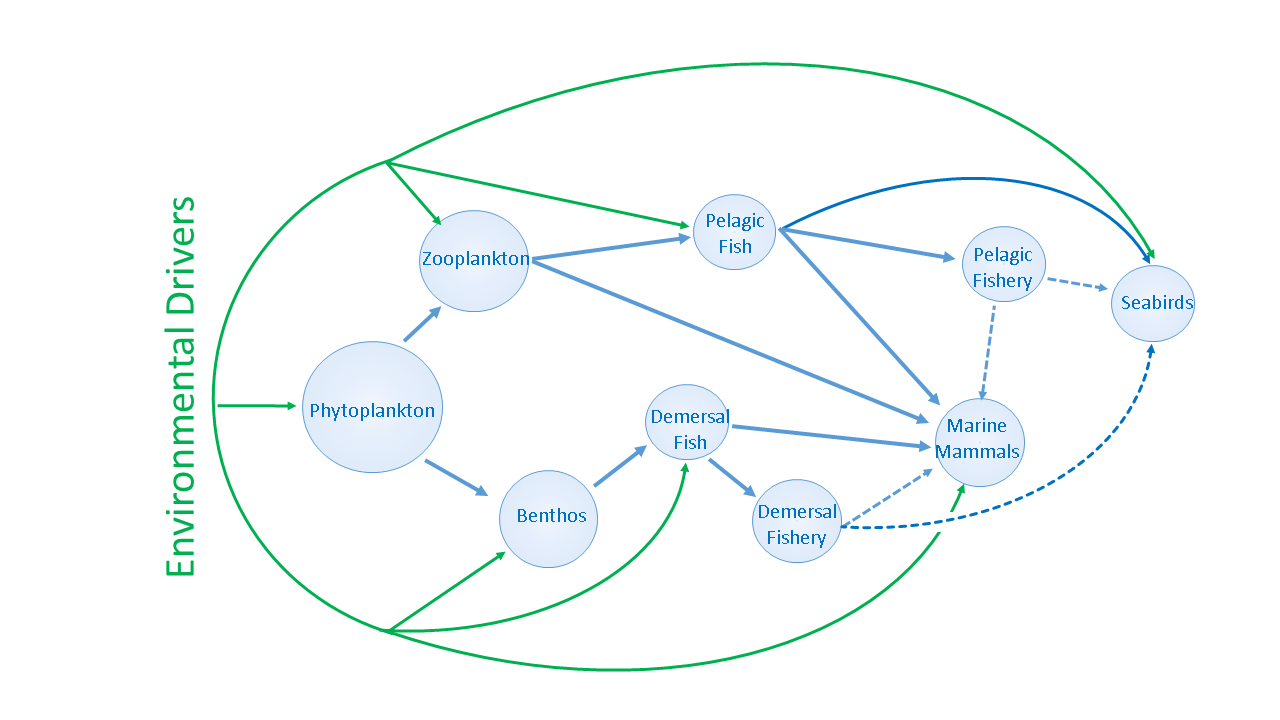
\includegraphics[width=\linewidth]{C:/Users/kimberly.bastille/Documents/GitHub/SOE-NEFMC/images/SOE_Network_Diagram} 

}

\caption{Simplified representation of the pathways linking primary production and environmental driver throughout a fishery ecosystem. The important societal benefits that derive from sustainable fisheries depend directly on a sequence of events starting at the base of the food web. The production of fish and shellfish available for harvest by the fisheries follows pathways of energy flow from phytoplankton and zooplankton to different parts of the food web. The production at each component further depends on the effect of a host of environmental drivers including temperature, salinity, and other factors.}\label{fig:prod-potential}
\end{figure}

There is a trend of increasing primary production in both New England
systems, primarily driven by increased summer production, which is due
to warmer temperatures and increased bacterial remineralization and
nutrient recycling (Fig. \ref{fig:NE-PP-OCCI}). This increased
productivity is most likely from smaller-celled species that contribute
less to fish production compared to larger phytoplankton. The 2018
winter-spring phytoplankton bloom, comprised primarily of larger
diatoms, was above average in both the GOM and GB, however the timing in
the GB was earlier than normal (Fig. \ref{fig:NE-chl-weekly}). Summer
biomass was below average throughout most of the region, while the fall
bloom was below average nearshore in the GOM and slightly above average
offshore and in parts of GB.

\begin{figure}

{\centering \includegraphics{SOE-NEFMC-2019_files/figure-latex/NE-PP-OCCI-1} 

}

\caption{Monthly primary production trends show the annual cycle (i.e. the peak during the summer months) and the changes over time for each month.}\label{fig:NE-PP-OCCI}
\end{figure}

\begin{figure}

{\centering \includegraphics{SOE-NEFMC-2019_files/figure-latex/NE-chl-weekly-1} 

}

\caption{Weekly chlorophyll concentrations and primary productivity for 2018 in Gulf of Maine and Georges Bank are shown by the colored lines in the above figures. The long-term mean is shown in black and shading indicates +/- 1 sample SD.}\label{fig:NE-chl-weekly}
\end{figure}

\subsection{Zooplankton (GOM and GB)}\label{zooplankton-gom-and-gb}

The most abundant zooplankton species in the GOM are \emph{Calanus
finmarchicus} (an important prey for larval fish and the north Atlantic
right whale), \emph{Centropages typicus}, and \emph{Psuedocalanus} spp.
{[}\protect\hyperlink{ref-morse_distinct_2017}{7}{]}. \emph{Calanus
finmarchicus} had low overall abundance in the GOM from 2009-2014, with
higher than normal abundance in 2015-2016 and a return to normal levels
in 2017 (Fig. \ref{fig:NE-zoo-abund}). On GB, \emph{Calanus
finmarchicus} annual abundance has been low continually since 2009.
\emph{Centropages typicus} has had higher than normal abundance from
2012-2017 on both GB and GOM. \emph{Pseudocalanus} abundance trends were
similar to \emph{Calanus} in recent years, with low abundance from
2001-2014 in the GOM and higher than normal 2015-2016, but normal
abundance in 2017. On GB, \emph{Pseudocalanus} abundance has a
significant long term decline (Fig. \ref{fig:NE-zoo-abund}) with an
increase to the long term mean in 2016-2017.

\begin{figure}

{\centering \includegraphics{SOE-NEFMC-2019_files/figure-latex/NE-zoo-abund-1} 

}

\caption{Abundance anomaly time series for key zooplankton species found in the GOM and GB.}\label{fig:NE-zoo-abund}
\end{figure}

Changes in the abundance of the larger \emph{Calanus finmarchicus} are
also reflected in the size distribution of the copepods. The small-large
copepod index is a measure of the relative size composition of the
dominant copepod taxa. During the 1990s and early 2000s, the positive
index was driven by high relative abundance of smaller bodied copepods
and a lower relative abundance of \emph{Calanus finmarchicus}. This
period also corresponds with regime shifts to lower fish recruitment
{[}\protect\hyperlink{ref-perretti_regime_2017}{3}{]}. The current trend
in the index suggests an increase in the relative abundance of smaller
bodied copepods (Fig. \ref{fig:NE-sli}).

\begin{figure}

{\centering \includegraphics{SOE-NEFMC-2019_files/figure-latex/NE-sli-1} 

}

\caption{GOM and GB small-large zooplankton index and the annual primary production anomaly.}\label{fig:NE-sli}
\end{figure}

Changes in primary productivity, phytoplankton and zooplankton
composition and abundance affect the food web and may be related to
observed changes in fish condition, recruitment patterns, and forage
fish energy content. However, more research and analyses are needed to
directly link these connections. Any attempt to predict how the
ecosystem will respond to changes in climate and fishing patterns
ultimately will depend on understanding these connections. Our objective
is to shed light on these fundamental issues and to document changes
affecting human communities and the fishery ecosystem on which we
depend.

\section{Contributors}\label{contributors}

\textbf{Editors} (NOAA NMFS Northeast Fisheries Science Center, NEFSC):
Sarah Gaichas, Sean Hardison, Scott Large, Sean Lucey

\textbf{Contributors} (NEFSC unless otherwise noted): Lisa Calvo
(Rutgers), Matthew Camisa (MA Division of Marine Fisheries), Patricia
Clay, Lisa Colburn, Geret DePiper, Michael Fogarty, Paula Fratantoni,
Kevin Friedland, Sarah Gaichas, James Gartland (Virginia Institute of
Marine Science), Heather Haas, Sean Hardison, Kimberly Hyde, Terry Joyce
(Woods Hole Oceanographic Institute), John Kosik, Steve Kress and Don
Lyons (National Audubon Societyas Seabird Restoration Program), Sean
Lucey, Chris Melrose, Ryan Morse, Kimberly Murray, Chris Orphanides,
Richard Pace, Charles Perretti, Karl Roscher (Maryland Department of
Natural Resources), Vincent Saba, Laurel Smith, Mark Terceiro, John
Walden, Harvey Walsh, Mark Wuenschel, and Qian Zhang (Unversity of
Maryland and US EPA Chesapeake Bay Program).

\newpage 

\section{Document Orientation}\label{document-orientation}

The figure format is illustrated in Fig \ref{fig:docformat}a. Trend
lines are shown when slope is significantly different from 0 at the p
\textless{} 0.05 level. An orange line signifies an overall positive
trend, and purple signifies a negative trend. To minimize bias
introduced by small sample size, no trend is fit for \textless{} 30 year
time series. Dashed lines represent mean values of time series unless
the indicator is an anomaly, in which case the dashed line is equal to
0. Shaded regions indicate the past ten years. If there are no new data
for 2018, the shaded region will still cover this time period. The
spatial scale of indicators is either coastwide, New England states
(Maine, New Hampshire, Massachusetts, Rhode Island, Connecticut), or at
the Gulf of Maine (GOM) and Georges Bank (GB) Ecosystem Production Unit
(EPU, Fig. \ref{fig:docformat}b) level.

\begin{figure}

{\centering \includegraphics{SOE-NEFMC-2019_files/figure-latex/docformat-1} 

}

\caption{Document orientation. a. Key to figures. b.The Northeast Large Marine Ecosystem.}\label{fig:docformat}
\end{figure}

Fish and invertebrates are aggregated into similar feeding categories
(Table \ref{tab:species-groupings}) to evaluate ecosystem level trends
in predators and prey.

\begin{table}[!h]

\caption{\label{tab:species-groupings}Feeding guilds and management bodies.}
\centering
\resizebox{\linewidth}{!}{
\fontsize{10}{12}\selectfont
\begin{tabular}{>{\raggedright\arraybackslash}p{2cm}>{\raggedright\arraybackslash}p{4cm}>{\raggedright\arraybackslash}p{2cm}>{\raggedright\arraybackslash}p{5cm}>{\raggedright\arraybackslash}p{6cm}}
\toprule
\textbf{Guild} & \textbf{MAFMC} & \textbf{Joint} & \textbf{NEFMC} & \textbf{State or Other}\\
\midrule
Apex Predator & NA & NA & NA & bluefin tuna, shark uncl, swordfish, yellowfin tuna\\
\cmidrule{1-5}
Piscivore & bluefish, summer flounder & goosefish, spiny dogfish & acadian redfish, atlantic cod, atlantic halibut, clearnose skate, little skate, offshore hake, pollock, red hake, silver hake, smooth skate, thorny skate, white hake, winter skate & fourspot flounder, john dory, sea raven, striped bass, weakfish, windowpane\\
\cmidrule{1-5}
Planktivore & atlantic mackerel, butterfish, longfin squid, northern shortfin squid & NA & atlantic herring & alewife, american shad, blackbelly rosefish, blueback herring, cusk, longhorn sculpin, lumpfish, menhaden, northern sand lance, northern searobin, sculpin uncl\\
\cmidrule{1-5}
Benthivore & black sea bass, scup, tilefish & NA & american plaice, barndoor skate, crab,red deepsea, haddock, ocean pout, rosette skate, winter flounder, witch flounder, yellowtail flounder & american lobster, atlantic wolffish, blue crab, cancer crab uncl, chain dogfish, cunner, jonah crab, lady crab, smooth dogfish, spider crab uncl, squid cuttlefish and octopod uncl, striped searobin, tautog\\
\cmidrule{1-5}
Benthos & atlantic surfclam, ocean quahog & NA & sea scallop & blue mussel, channeled whelk, sea cucumber, sea urchin and sand dollar uncl, sea urchins, snails(conchs)\\
\bottomrule
\end{tabular}}
\end{table}

\newpage 

\section*{References}\label{references}
\addcontentsline{toc}{section}{References}

\hypertarget{refs}{}
\hypertarget{ref-zhang_role_2007}{}
1. Zhang R, Vallis GK. The Role of Bottom Vortex Stretching on the Path
of the North Atlantic Western Boundary Current and on the Northern
Recirculation Gyre. Journal of Physical Oceanography. 2007;37:
2053--2080.
doi:\href{https://doi.org/10.1175/JPO3102.1}{10.1175/JPO3102.1}

\hypertarget{ref-goddard_extreme_2015}{}
2. Goddard PB, Yin J, Griffies SM, Zhang S. An extreme event of
sea-level rise along the Northeast coast of North America in 2009--2010.
Nature Communications. 2015;6.
doi:\href{https://doi.org/10.1038/ncomms7346}{10.1038/ncomms7346}

\hypertarget{ref-perretti_regime_2017}{}
3. Perretti C, Fogarty M, Friedland K, Hare J, Lucey S, McBride R, et
al. Regime shifts in fish recruitment on the Northeast US Continental
Shelf. Marine Ecology Progress Series. 2017;574: 1--11.
doi:\href{https://doi.org/10.3354/meps12183}{10.3354/meps12183}

\hypertarget{ref-greene_remote_2013}{}
4. Greene CH, Meyer-Gutbrod E, Monger BC, McGarry LP, Pershing AJ,
Belkin IM, et al. Remote climate forcing of decadal-scale regime shifts
in Northwest Atlantic shelf ecosystems. Limnology and Oceanography.
2013;58: 803--816.
doi:\href{https://doi.org/10.4319/lo.2013.58.3.0803}{10.4319/lo.2013.58.3.0803}

\hypertarget{ref-hare_vulnerability_2016}{}
5. Hare JA, Morrison WE, Nelson MW, Stachura MM, Teeters EJ, Griffis RB,
et al. A Vulnerability Assessment of Fish and Invertebrates to Climate
Change on the Northeast U.S. Continental Shelf. PLOS ONE. 2016;11:
e0146756.
doi:\href{https://doi.org/10.1371/journal.pone.0146756}{10.1371/journal.pone.0146756}

\hypertarget{ref-pace_statespace_2017}{}
6. Pace RM, Corkeron PJ, Kraus SD. State--space mark--recapture
estimates reveal a recent decline in abundance of North Atlantic right
whales. Ecology and Evolution. 2017;7: 8730--8741.
doi:\href{https://doi.org/10.1002/ece3.3406}{10.1002/ece3.3406}

\hypertarget{ref-morse_distinct_2017}{}
7. Morse R, Friedland K, Tommasi D, Stock C, Nye J. Distinct zooplankton
regime shift patterns across ecoregions of the U.S. Northeast
continental shelf Large Marine Ecosystem. Journal of Marine Systems.
2017;165: 77--91.
doi:\href{https://doi.org/10.1016/j.jmarsys.2016.09.011}{10.1016/j.jmarsys.2016.09.011}


\end{document}
